\subsection{Scalability}
\label{sec:res_scale}

Our planner solves the OCP~\eqref{eq:ocp} with a fixed number of sequential-quadratic-programming (SQP) iterations
per 100\,ms tick, warm-started from the previous plan. Fewer iterations shorten the tick but leave the plan short of
convergence. We measure what that costs against the fleet size in two ways. In closed loop, the four-carrier twin
flew a hover, the figure-eight at 0.2\,m/s and an unannounced release, each from a floor start, at one iteration and
at five. Offline, each plan at one and two iterations was compared with the plan converged from the same iterate. The
bars of both checks were fixed before the runs: the dynamics residual of the plan, the error of the references the
trackers fly at the next node and the fifth, the error of the thrust feed-forward, and the cost's ratio to the
converged plan's.

In closed loop at four carriers, one iteration a tick flew as well as five in every cell. The ring's path error and
tilt stayed inside the bars set from the five-iteration runs through the lift, the path and the release, and no run
dropped, aborted or failed a solve. The plans were not converged, however: their dynamics residual peaked at the
release, under the closed loop's limit but over the offline bar.

Offline, the answer depends on the fleet. Replayed tick by tick, nine recorded flights with two to four carriers, the
rig's among them, converge by every bar at two iterations; at one iteration every rig flight breaks the residual bar.
At eight carriers on the figure-eight, with each warm start moved off the plan by about the rig's ring error, one
iteration misses every bar, two miss only the feed-forward bar (0.316 against 0.3\,m/s$^2$), and five pass all of
them (Table~\ref{tab:quality}, Fig.~\ref{fig:quality}). The iteration count must therefore grow with the fleet: two
suffice up to four carriers, while eight need five.

\begin{table}[t]
\centering
\footnotesize
\setlength{\tabcolsep}{4pt}
\caption{Plan quality at eight carriers against SQP iterations per tick: the figure-eight at 0.2\,m/s, each warm
start 1\,cm and 10\,cm/s off the plan, compared with the plan converged from the same iterate; 95th percentiles over
200 ticks. Bold: over the bar. No solve failed.}
\label{tab:quality}
\begin{tabular}{lcccc}
\toprule
Measure & Bar & 5 & 2 & 1 \\
\midrule
Cost ratio, median / 95th pct. & 1.10 / 1.50 & 1.000 / 1.001 & 1.003 / 1.010 & \textbf{miss}$^a$ \\
Dynamics residual & $10^{-3}$ & $3.2{\times}10^{-7}$ & $8.8{\times}10^{-5}$ & $\mathbf{9.3{\times}10^{-3}}$ \\
Reference, node 1 / 5 (mm) & 5 / 10 & 0.9 / 0.9 & 3.2 / 5.1 & \textbf{7.3} / \textbf{14.5} \\
Feed-forward (m/s$^2$) & 0.3 & 0.12 & \textbf{0.316} & \textbf{0.60} \\
\bottomrule
\multicolumn{5}{p{0.95\columnwidth}}{\footnotesize $^a$\,170 of 200 ticks over the residual bar, each counted as a
miss.}
\end{tabular}
\end{table}

\begin{figure}[t]
\centering
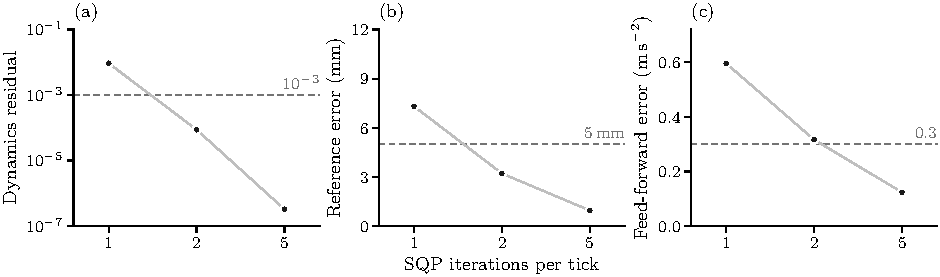
\includegraphics[width=\columnwidth]{figures/fig_s_quality_n8.pdf}
\caption{Plan quality at eight carriers against SQP iterations per tick, relative to the converged plan: the
dynamics residual, the reference error at the next node and the thrust feed-forward error (95th percentiles), with
the bars fixed before the runs. One iteration misses every bar, two miss only the feed-forward bar, five pass.}
\label{fig:quality}
\end{figure}

What this means for real time is set by the slowest tick. On the rig laptop, a bench calibrated against the rig's own
flights gives the largest team our planner flies within the 100\,ms period at five iterations as
\placeholder{$N_{\max}$ on the rig laptop at 5 iterations, from the bench with the speed-ups and the pivot}. At
eight carriers the plan must be read at five iterations, which the rig laptop cannot run in real time; the
eight-carrier results are therefore the twin's, with its clock slowed, and say nothing about real time. In the twin,
eight carriers lifted a larger ring from the floor and carried it through four unannounced releases, in opposite
pairs, to a square of four and back to eight by rejoins (Fig.~\ref{fig:s_chain}), with the ring's tilt peaking at a few
degrees and no drop. \placeholder{the eight-carrier claim runs at 5 iterations, hover and $8 \to 4 \to 8$, two each:
ring position error and tilt peak with the team back at eight, scored from 2\,s after the last rejoin's blend ends;
release tilt peak; achieved real-time factor and late ticks}.
